% main.tex - Updated Research Template with new title page
\documentclass{research}

\usepackage{graphicx} %LaTeX package to import graphics
\graphicspath{{images/}} %configuring the graphicx package

\usepackage{ragged2e} % Add this to your preamble
\usepackage{tikz}
\usepackage{caption}
\usepackage{pdflscape}
\usepackage{amsmath}
\usepackage{booktabs}
\usepackage{array}
\usepackage{float}

% Title Page Info
\title{}
\author{Fritzgerald Enric T. Imperial}
\submission{A Special Project Presented to the Faculty of the College of Computer Studies, Naga College Foundation, Inc., Naga City}
\researchyear{2026}

\begin{document}

% Generate Title Page
\thispagestyle{empty}
\begin{center}
  \vspace*{1in}
  {\Huge\bfseries Intelligent Queue Management System for Wait Time Transparency \par}
  \vspace{1in}
  A Capstone Project\\
  Presented to the Faculty of the\\
  College of Computer Studies\\
  Naga College Foundation, Inc.\\
  Naga City\\
  \vspace{1in}
  In Partial Fulfillment of\\
  The Requirements for the Degree\\
  Bachelor of Science in Information System\\
  \vspace{0.5in}
  Kemuel Dave P. Alcebor\\
  Adolf Rey Asagra\\
  Paolo Eavan Z. Barcinas\\
  Terence Joshua De Vega\\
  Ehrvayn Rayven Olivera\\
  \vspace*{0.5in}
  2026
\end{center}
\clearpage

% -------------------------------------------------------
% FIX 1: \chapter*{} is now closed immediately.
%         \pagestyle{empty} is placed AFTER the command.
%         All bare \vspace replaced with \vspace{0.3in}
% -------------------------------------------------------


\tableofcontents

\clearpage

\listoffigures

\clearpage

\listoftables

\clearpage

%-----------------------------
% Chapter 1
%-----------------------------
\chapter{Introduction}

\section{Background of the Study}

\indent Higher education institutions across the world continue to embrace digital transformation to enhance administrative efficiency and student experience. Despite these advancements, many universities and colleges in the Philippines—particularly in the Bicol Region—still rely heavily on traditional, manual queuing practices. In our own home institution, we have repeatedly observed long lines forming as early as opening hours, congested waiting areas, and students anxiously crowding service windows just to confirm their queue status. These conditions have become a familiar scene every enrollment period and during peak payment schedules, showing how outdated queuing processes create visible disruptions in the normal flow of campus operations.

From our firsthand experiences as students, the lack of transparency in waiting times is one of the most frustrating issues. Students often wait for an uncertain period with no idea of how many people are still ahead of them or when they might finally be served. Many return multiple times to check their number manually or, worse, miss their turn because no announcement system is in place—an observation consistent with findings from other Philippine HEIs that highlight inefficiencies in manual queueing practices \cite{ref51}. During high-volume periods such as enrollment and cashiering, these issues intensify, leading to overcrowding, delays, and heightened student stress—similar to trends reported by \cite{ref87} regarding service bottlenecks in public and educational institutions.

These institutional challenges place pressure not only on students but also on administrative personnel. Staff members face difficulty tracking the volume of students, coordinating service flow, and managing records while addressing repeated inquiries from students waiting in line. Research shows that manual queue management significantly reduces staff productivity and increases processing errors \cite{ref39}. Such patterns closely mirror the inefficiencies we have witnessed firsthand within our home institution, especially during enrollment and financial transactions.

Most institutions in Bicol, like ours, continue to use manual or semi-digital queueing setups that lack automation, real-time updates, and predictive capabilities. Without smart features such as automated notifications, queue tracking, or estimated wait-time predictions, miscommunication frequently occurs between personnel and students—resulting in wasted time and dissatisfaction. Studies have emphasized that queue transparency and automated service alerts can substantially improve user experience and reduce congestion \cite{ref88}, reinforcing the need for modernization.

Globally and nationally, higher education is moving toward smart-campus strategies aligned with computer vision, automation, and data-driven intelligence. Modern queue management systems integrating Computer Vision (CV) detection, AI predictions, and mobile-based alerts have proven effective in improving real-time service flow and reducing student wait times \cite{ref89}. If implemented in Bicol institutions, such innovations could significantly enhance service delivery, support operational efficiency, and align local campuses with current smart-campus trends.

Recognizing the persistent issues that we personally experienced and observed—congestion, uncertainty, and delays—we believe that developing an Intelligent Queue Management System with Wait-Time Transparency is both timely and essential. By integrating real-time monitoring through Computer Vision technology, automated alerts, and predictive analytics, the proposed system aims to address the long-standing problems associated with manual queueing. Ultimately, this research seeks to improve the overall queue experience for students, streamline administrative workflows, and contribute to the institution's broader digital transformation efforts.

\section{Review of Related Literature}
\subsection{Impact of Intelligent QMS on Customer Satisfaction}

A Queue Management System (QMS) is a conceived system that is used to manage service lines, control the movement of customers, and offer a formalized control of the waiting process in either a physical or digital service call center. Intelligent QMS models that are modern incorporate automation, data analytics, and real-time information delivery to increase transparency, efficiency, and the overall user experience.

Quality Management Systems (QMS) play a significant role in assuring the uniformity of product and service quality, a factor that significantly influences customer satisfaction \cite{ref6},\cite{ref7},\cite{ref8},\cite{ref9}. Empirical research across the construction, manufacturing, and service industries demonstrates that an effective QMS enhances process reliability, operational efficiency, and service consistency, thereby bolstering customer trust and loyalty \cite{ref3},\cite{ref10},\cite{ref11}. In the context of Industry 4.0 technologies, intelligent QMS, referred to as Quality 4.0, incorporates automation, Artificial Intelligence (AI), and Computer Vision (CV)-based monitoring systems, alongside real-time analytics, to proactively monitor and enhance quality \cite{ref12},\cite{ref13},\cite{ref14},\cite{ref15}.

Such systems augment traceability, control, and responsiveness, thereby enriching customer experiences \cite{ref16},\cite{ref17},\cite{ref18}.

AI-enabled analytical frameworks, together with Computer Vision–based detection and digital feedback mechanisms, facilitate organizations in forecasting and mitigating service and quality-related challenges, thereby augmenting uniformity and user satisfaction \cite{ref19},\cite{ref20},\cite{ref21},\cite{ref22}. Strategies centered on customer engagement within sophisticated Quality Management Systems (QMS), encompassing real-time monitoring through Computer Vision, tailored service flow control, and continuous feedback mechanisms, significantly bolster customer satisfaction and system efficiency \cite{ref23},\cite{ref24},\cite{ref25},\cite{ref26}.

ISO 9001 certification and structured QMS frameworks ensure standardized processes and measurable improvements, supporting customer satisfaction \cite{ref27},\cite{ref6},\cite{ref7}. However, studies directly measuring full-scale intelligent QMS impact on satisfaction remain limited, especially in service sectors integrating Computer Vision–based queue monitoring and prediction systems \cite{ref28},\cite{ref19},\cite{ref21},\cite{ref18},\cite{ref29},\cite{ref20}. Your study addresses this gap by examining how intelligent QMS with Computer Vision capabilities affects user satisfaction, offering both practical and theoretical insights \cite{ref6},\cite{ref9},\cite{ref3}.

Intelligent Queue Management Systems integrate Computer Vision technology, structured processes, and customer-focused strategies to enhance quality, consistency, and responsiveness. Although the advantages pertaining to user satisfaction are apparent, empirical investigations regarding full Computer Vision–based queue implementation are still limited, thereby underscoring the significance of research endeavors such as yours that examine the direct influence of intelligent QMS on user experience.

\subsection{Business Intelligence (BI) Systems for Dynamic Demand Matching}
Business Intelligence BI is a combination of technologies, processes, and analysis that are applied to gather, combine, and analyze organizational data in order to make informed decisions. BI systems use data analytics, reporting tools, and visualization platforms to convert raw operating information into actionable information so that an organization can discover patterns, help predict demand variability and can optimize resource allocation in real-time.

Business Intelligence BI systems are significantly important for helping companies make smart decisions based on data and boost their overall performance in every industry \cite{ref42}, \cite{ref43}, \cite{ref44}, \cite{ref45}. Using BI tools that mix analytics, dashboards, and reporting lets businesses keep an eye on trends, guess what is going to happen next, and jump on changes fast when demand spikes \cite{ref46}, \cite{ref48}, \cite{ref49}, \cite{ref50}.

The application of artificially intelligent systems and machine learning gives better BI through the use of predictive analytics, real-time insights, and automated decision support, which would further refine the accuracy in demand forecasting and resource distribution \cite{ref57}, \cite{ref68}, \cite{ref42}, \cite{ref56}. The joining up with the Internet of Things IoT platforms in this regard allows for easier monitoring, data gathering, and dynamic changes especially in difficult systems \cite{ref41}, \cite{ref69}. AI systems and machine learning improve Business Intelligence with predictive analytics, real-time insights, and automatic decisions. This makes demand forecasting and resource sharing more accurate. Connecting with Internet of Things platforms also makes monitoring, data collection, and quick changes easier, even in complex systems.

BI systems on the other hand also render customer segmentation, personalizing strategies, and compliance monitoring, contributing to organizational agility \cite{ref49}, \cite{ref62}, \cite{ref59}. The cloud-based solutions provide more accessibility, scalability, and security thus organizations are able to react more quickly to market changes \cite{ref52}, \cite{ref60}, \cite{ref67}.

Furthermore, BI supports cross-departmental coordination and supply chain optimization, linking analytics with process performance to maintain competitiveness \cite{ref63}, \cite{ref66}, \cite{ref47}. In sectors such as manufacturing, finance, energy, and emergency services, BI-driven decisions improve resilience, efficiency, and strategic planning \cite{ref40}, \cite{ref58}, \cite{ref41}.

Business Intelligence BI systems turn raw data into useful information that helps match demand, improve how things run, and make smart decisions. Using AI, machine learning, and IoT, BI can predict future trends and make quick changes when needed and this is crucial in cloud technology and teamwork across departments because it makes BI easier to use and stronger. Also, when set up well and linked to company goals, BI brings the best results. Overall, BI helps businesses prepare for demand, work better, and stay ahead in changing markets \cite{ref42}, \cite{ref69}, \cite{ref50}, \cite{ref80}.

\subsection{UI/UX Design Principles for Public Information Displays }
The principles of User Interface (UI) and User Experience (UX) are the guidelines in developing digital interfaces that are intuitive, clear, and effective for the end-user. UI focuses on the visual and interactive aspects of a system, whereas UX emphasizes usability, intelligibility, and satisfaction during user interaction. These design principles are crucial in public information displays, where users must quickly understand information, navigate seamlessly, and experience reduced cognitive load while accurately interpreting service updates \cite{ref54},\cite{ref55}.

Recent studies on UI/UX design in queue management displays, public notifications, kiosks, and real-time information systems have grown significantly since 2020. Research highlights the influence of screen layout elements such as size, contrast, text style, and placement on user attention and comprehension \cite{ref54}. Interactive features like gestures, touch, and proximity can increase engagement and attention, but excessive complexity may cause cognitive overload \cite{ref56},\cite{ref57},\cite{ref58}.

Another body of literature emphasizes feedback mechanisms to reduce perceived waiting time and user anxiety, including countdown timers, progress indicators, loading states, and context-sensitive alerts \cite{ref59},\cite{ref60},\cite{ref61}. Visualizing unavoidable delays through animated placeholders or staged content helps maintain user trust, while predictive displays require accurate frequency of updates and error margins for fairness and transparency \cite{ref62},\cite{ref63},\cite{ref53}. Multimodality, accessibility, and human-centered design form another key focus. Studies show that large touchscreens, simplified navigation, familiar metaphors, redundant notification systems, ethical data practices, and privacy protection foster more inclusive and equitable queueing experiences \cite{ref54},\cite{ref55},\cite{ref38},\cite{ref64},\cite{ref62},\cite{ref4}.

Other research demonstrates that integrating real-time information systems with AI and Computer Vision improves adaptability, predictive accuracy, and overall performance of queue management systems \cite{ref64},\cite{ref65},\cite{ref66},\cite{ref67},\cite{ref68},\cite{ref56},\cite{ref53},\cite{ref69},\cite{ref54}. These studies collectively highlight the importance of legibility, visual hierarchy, timely feedback, accessibility, and modular system architecture. Implementing iterative, user-driven design and pilot-based validation ensures that a Computer Vision–enabled, AI-assisted queue management system can deliver measurable improvements to both process efficiency and user experience \cite{ref56},\cite{ref61},\cite{ref59},\cite{ref63},\cite{ref55},\cite{ref65}.


\section{Synthesis of the State-of-the-Art}

\indent QMS have developed into all-round solutions, which optimize the customer flow, efficiency, and quality of services. Current smart QMS combine automation, analytics, and real-time delivery of information to make waiting processes transparent and enhance them. The integration of Quality Management Systems, Business Intelligence tools, and UI/UX design has only enlarged the ability of QMS to be able to support efficient operations and increase customer satisfaction. Together, the recent literature emphasizes that integrated, data-driven, and user-centered systems and which enable consistent service delivery are needed. Nevertheless, with increasing technology, the empirical studies that assess the holistic effect of intelligent QMS, especially in educational and service driven organizations, have been limited and thus the study fills significant gaps.

Quality Management Systems QMS are considered t o play a vital role in providing uniformity, dependability, and efficiency of products and services. In all industrial sectors, research indicates that the successful implementation of QMS enhances customer satisfaction by increasing the reliability of the process, process control, and process uniformity \cite{ref8} \cite{ref13} \cite{ref23} \cite{ref19}. The empirical research proves that a strong QMS model leads to improvement of the level of customer trust and loyalty, particularly when the operational processes are standardized and reviewed on a regular basis \cite{ref39} \cite{ref14} \cite{ref25}. Several years later, with the advent of Industry 4.0 technologies, Quality 4.0 considers Computer Vision (CV), AI, automation, and real-time analytics as part of the QMS structures and enhances responsiveness, traceability, and proactive quality assurance \cite{ref7} \cite{ref34} \cite{ref31} \cite{ref17}. It is these systems that enhance organizational abilities to control service settings, to address operational issues, and to enhance the customer experience \cite{ref37} \cite{ref29} \cite{ref85}. The predictive opportunities and the ability to expect and solve the quality-related challenges caused by AI-based feedback mechanisms also increase service consistency and customer satisfaction \cite{ref55} \cite{ref10} \cite{ref11} \cite{ref18} \cite{ref6}. Even standardized frameworks like ISO 9001 have shown quite tangible increases in customer satisfaction, but studies on the complete smart implementation of a QMS, particularly in the real-world service, are limited  \cite{ref15} \cite{ref36} \cite{ref26}.

Business Intelligence BI systems assist the organizations, converting the data regarding their operations into the actionable information needed to make the decisions in the real-time and match the demand dynamically. The sources define BI as a key factor that allows organizations to understand trends, forecast fluctuations, and better use resources \cite{ref42} \cite{ref43} \cite{ref44} \cite{ref45}. BI allows making organizations responsive and agile to changing demand by combining analytics, dashboards, and reporting tools \cite{ref46} \cite{ref48} \cite{ref49} \cite{ref50}. AI and machine learning enhance the BI potential through enhanced predictive accuracy and automation of decision-making processes of a complex nature \cite{ref57} \cite{ref68} \cite{ref56}. By linking to Computer Vision systems, BI systems enhance further the monitoring, data gathering, and real-time operational modifications \cite{ref41} \cite{ref69}. Other benefits such as improved customer segmentation, personalization, compliance monitoring, and better organizational performance are all improved \cite{ref62} \cite{ref59}. Cloud-based BI systems can help organizations to react efficiently to the evolving rapidly changing environments and to be scalable, accessible, and secure \cite{ref60} \cite{ref67}. It is also demonstrated that BI enhances cross-departmental coordination, supply chain performance, and strategic planning at a wide range of spheres, including manufacturing, finance, and emergency services \cite{ref63} \cite{ref66} \cite{ref58}. Such findings indicate the importance of BI in enabling demand forecasting, operational optimization, and evidence-based decision making -functions that are essential to contemporary queue management systems.

UI/UX design principles are critical in determining how the users will interact with the information displays and queue management systems that are accessible in the public. Researchers highlight that visual hierarchy, legibility, contrast, the screen size, and display structure are important factors that determine user attention and understanding especially in busy service settings  \cite{ref20}. Interaction features like touch, gestures, proximity, and other characteristics improve interaction and need to be intuitive to prevent cognitive overload \cite{ref70} \cite{ref72}. The studies of feedback mechanisms emphasize the significance of countdown timers, progress indicators, and predictive notifications in terms of shortening the perceived waiting time and user anxiety \cite{ref78} \cite{ref71}. The research in the field of human-computer interaction also proves that by visualizing the inevitable delays with the help of animated placeholders or staged content, the user trust is preserved, as long as updates are timely and estimations are accurate \cite{ref80} \cite{ref24} \cite{ref79}. There is yet another important literature that highlights or not only the importance of accessibility and inclusiveness by providing multimodal interfaces, simplifying navigation, redundant notifications, ethical data practices, or privacy-protective design \cite{ref20} \cite{ref21} \cite{ref57}. The literature, as a whole, confirms that there is a set of design principles that intelligent queue management systems should follow: interfaces need to be extremely readable, feedback should be timely and contextually relevant, and systems should be accessible to both digitally literate and digitally underserved groups.

\section{Gap Bridged by the Study}
While literature emphasizes automation, real-time analysis, and user-centered design across Quality Management Systems, Business Intelligence, and UI/UX domains, research integrating these elements into intelligent queue management remains limited, particularly regarding multi-office coordination, wait-time transparency with predictive communication, the operational impact of predictions beyond algorithmic accuracy, accessibility for diverse digital literacy levels, mixed-method evaluation combining quantitative service metrics with qualitative user experience data, and privacy-by-design principles.

This study addresses these gaps by developing an Intelligent Queue Management System that unifies Computer Vision (CV)-based sensing, AI- and BI-driven wait-time prediction, and inclusive UI/UX design within a single prototype spanning Enrollment and Cashier services, incorporating privacy protection, predictive decision-making rules, and a comprehensive evaluation framework to assess its impact on wait-time transparency, operational efficiency, and user satisfaction.

\section{Theoretical Framework}
This study's theoretical foundation rests upon four interconnected frameworks: Queueing Theory by Agner Krarup Erlang. Human-Computer Interaction or HCI Theory by Vannevar Bush, Douglas Engelbart, and Ben Shneiderman, as cited by Gentile et al. \cite{ref70} and Information Systems Success Theory by Fred D. Davis, as cited by Tan, Leow, and Ong \cite{ref73}.
Queuing Theory, which provides the mathematical models for analyzing service flows and predicting Estimated Wait Times EWT; Information Transparency Theory \cite{ref71}, which asserts that communicating this EWT reduces user anxiety and builds trust; the Business Intelligence BI and Data-Driven Decision-Making paradigm, which utilizes analyzed data and AI-generated predictions to support dynamic resource allocation for administrators; and finally, Human–Computer Interaction HCI / UI-UX Design Principles \cite{ref70}, which ensure that transparent queue information is delivered through interfaces such as displays and notifications that are clear, accessible, and user-friendly.

First, Queuing Theory describes how arrival rates, service rates, and system utiliation influence waiting times and overall queue behaviour, forming the mathematical foundation for analyzing and optimizing service flows. Recent data-driven advancements, such as those demonstrated by Li et al., show how real-time data and predictive modelling can refine wait-time estimation and enable dynamic counter allocation. This makes Queuing Theory vital to the study, as it provides the quantitative basis for predicting congestion, reducing delays, and improving resource management in the proposed system.

Second, Information Transparency Theory highlights that the timeliness, clarity, and consistency of information reduce user uncertainty and enhance perceived fairness and satisfaction during waiting periods. Empirical evidence from \cite{ref71} shows that frequent and visible updates such as countdowns and estimated wait times significantly decrease users’ perceived waiting time. This underscores the importance of ensuring that the system delivers real-time information across multiple channels to maintain transparency and improve the overall waiting experience.

Third, the Technology Acceptance Model TAM is a framework that explains how users adopt new technology, emphasizing that perceived usefulness and perceived ease of use are key predictors of system adoption. In this study, TAM is important because it helps evaluate whether students and staff are likely to accept the smart queue management system, guiding improvements in design and implementation to ensure higher usability and engagement.

Finally, Human-Computer Interaction HCI and UI/UX Design principles assure the accessibility, intuition and cognitive effectiveness of interfaces; recent research by Gentile et al.,\cite{ref70} has shown how effective the hierarchy of information, visibility, and user-focused interaction design make interfaces easier to understand and interact with, which directly drives our queue displays, notification style and general user interface layout. All of these four theories combine to create an operational modelling, transparency communication, behavioural adoption and usability design theory, to create a complete theoretical base of a modern intelligent and student centered queue management system.

Together, these frameworks provide a unified foundation for the study. Queueing Theory supports the system’s predictive functions; Information Transparency Theory guides how wait-time data is communicated; TAM explains user adoption; and HCI/UI-UX principles ensure clear and accessible interfaces. Combined, they justify the system’s design, functionality, and user-centered approach.

\begin{figure}[htbp]
    \centering
    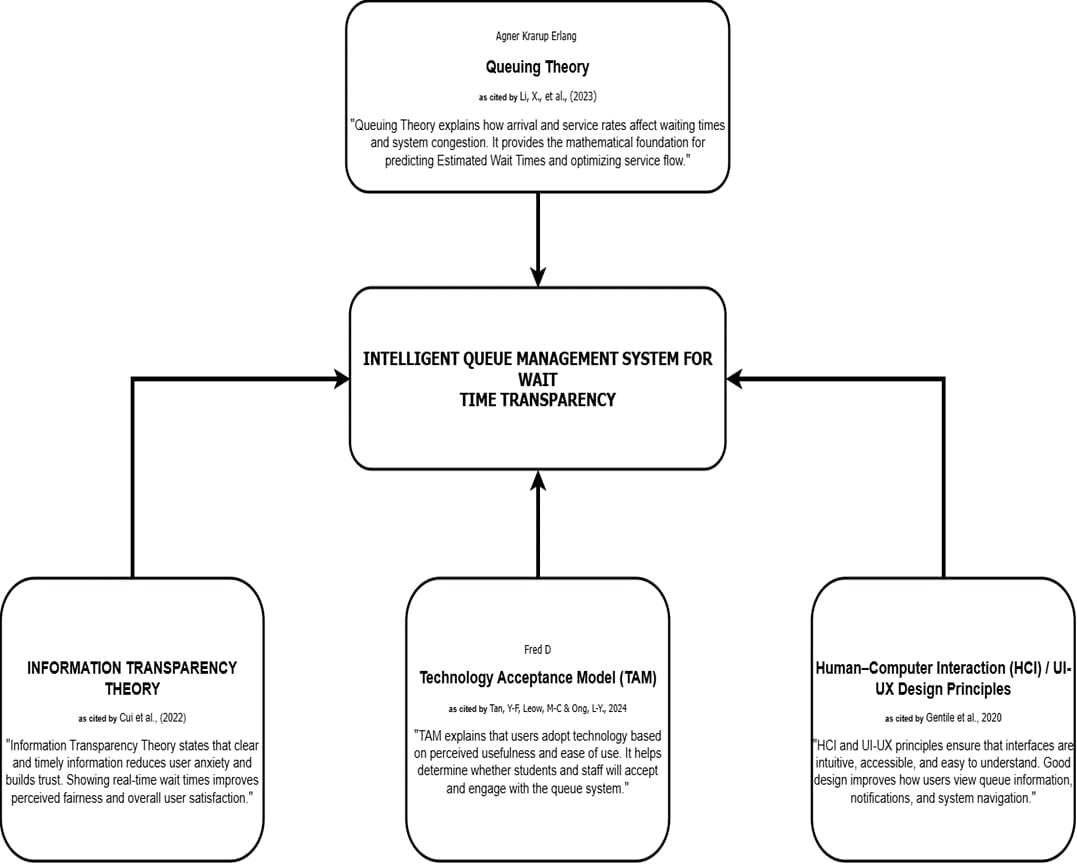
\includegraphics[width=0.9\textwidth, height=0.6\textheight, keepaspectratio]{image/Theoretical Diagram.jpg}
    \caption{Theoretical Framework}
    \label{fig:theoretical-framework}
\end{figure}

\vspace{0.5em}

\indent{This paper is grounded on four current theories which together provide the analytical, behavioral, and design foundations of the Intelligent Queue Management System for wait-time transparency.}

\section{Conceptual Framework}

The conceptual framework illustrates the Input, Process, Output, Outcome (IPOO) paradigm of this study. It shows how the proposed Intelligent Queue Management System for Wait Time Transparency enhances service efficiency and user experience across key campus departments. It explains how various inputs, such as human resources, Computer Vision (CV) devices, AI algorithms, and institutional data, are transformed through monitoring, analytics, and automated queue workflows to produce measurable outputs and long-term outcomes.

\indent\textbf{Input Stage.} The Input stage identifies the essential resources required to design, develop, and implement the Intelligent Queue Management System for Wait Time Transparency. These include: (1) Human resources, including BSIS student developers, school administrators, and personnel responsible for system construction, deployment, and maintenance. (2) Technological devices including Computer Vision (CV) cameras, QR code scanners, Microsoft Visio for modeling, and microcontrollers used for real-time data capture. (3) AI algorithms, which forecast queue lengths, optimize service allocation, and analyze operational data. (4) Institutional inputs, including data from enrollment and cashiering, along with relevant policies and workflows. (5) Infrastructure, which includes necessary hardware and software to support system operation. Together, these inputs enable the creation of an intelligent, responsive, and data-driven queue management solution.

\indent\textbf{Process Stage.} The Process stage describes activities that transform inputs into outputs. Key activities include: (1) Registration of queues and issuance of digital tickets via kiosks, web portals, or mobile applications. (2) Real-time data collection using Computer Vision (CV) cameras to monitor queue length, service times, and crowd flow. (3) AI-driven analysis to forecast waiting times, optimize counter assignments, and suggest operational adjustments. (4) Visualization and monitoring through dashboards, allowing administrators to track service performance and resource utilization. (5) Feedback integration and performance evaluation to ensure continuous system improvement. This stage ensures that the queue management system operates intelligently, responds dynamically to demand, and improves operational efficiency.

\indent\textbf{Output Stage.} The Output stage reflects immediate results from the system processes, including: (1) Automation and streamlining of campus service operations, reducing reliance on manual queueing. (2) Shorter response times and minimized congestion during peak periods. (3) Improved coordination, transparency, and communication across Enrollment and Cashiering services. (4) Enhanced user satisfaction through real-time notifications, estimated wait times, and clear service updates.

\indent\textbf{Outcome Stage.} The Outcome stage represents long-term institutional benefits achieved through consistent system deployment, including: (1) Increased operational efficiency, transparency, and service quality. (2) Data-driven decision-making using AI and analytics to plan, predict, and improve future operations. (3) Encouragement of digital innovation and adoption of Computer Vision and AI technologies aligned with institutional and national digital transformation goals. (4) Contribution to broader Smart Campus initiatives, fostering sustainability, technological advancement, and user-focused innovation.

Overall, the conceptual framework demonstrates how the integration of human, technological, and informational resources can produce an Intelligent Queue Management System for Wait Time Transparency that is efficient, inclusive, and capable of improving both operational performance and user experience across campus service.

\begin{figure}[htbp]
\centering

\scalebox{0.78}{%
\begin{minipage}{\textwidth}
\centering

\textbf{\large INTELLIGENT QUEUE MANAGEMENT SYSTEM FOR WAIT-TIME TRANSPARENCY}

\vspace{1em}

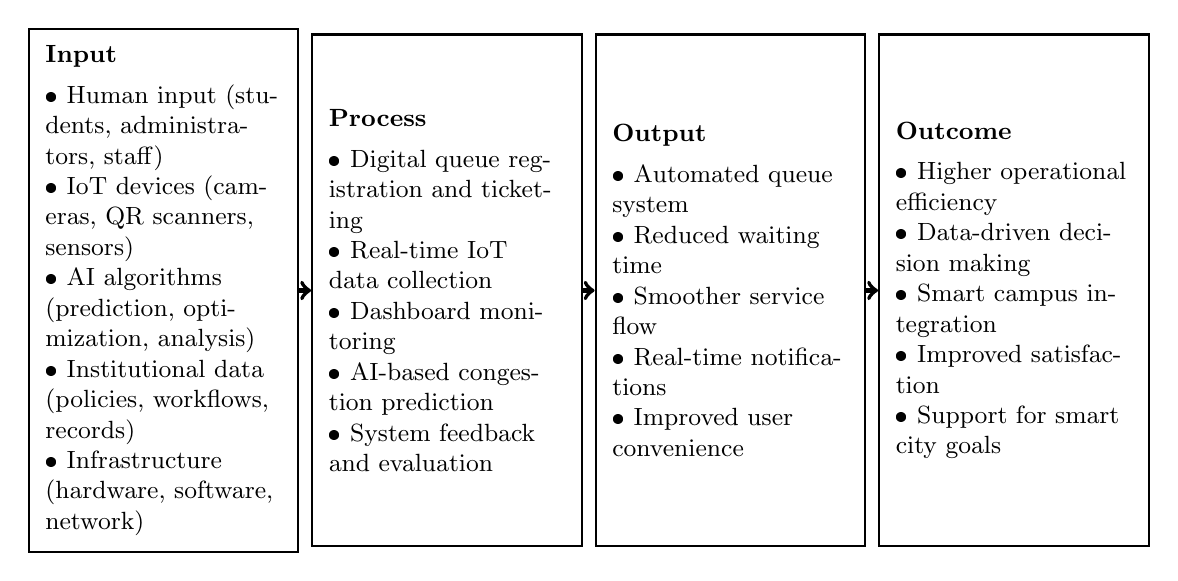
\begin{tikzpicture}[
    box/.style={
        rectangle,
        draw=black,
        thick,
        minimum width=3.2cm,
        minimum height=6.5cm,
        text width=3cm,
        align=left,
        font=\small,
        inner sep=6pt
    },
    arrow/.style={->, thick, line width=1.5pt}
]

\node[box] (input) at (0,0) {
\textbf{Input}\\[0.4em]
\textbullet\ Human input (students, administrators, staff)\\
\textbullet\ IoT devices (cameras, QR scanners, sensors)\\
\textbullet\ AI algorithms (prediction, optimization, analysis)\\
\textbullet\ Institutional data (policies, workflows, records)\\
\textbullet\ Infrastructure (hardware, software, network)
};

\node[box] (process) at (3.6,0) {
\textbf{Process}\\[0.4em]
\textbullet\ Digital queue registration and ticketing\\
\textbullet\ Real-time IoT data collection\\
\textbullet\ Dashboard monitoring\\
\textbullet\ AI-based congestion prediction\\
\textbullet\ System feedback and evaluation
};

\node[box] (output) at (7.2,0) {
\textbf{Output}\\[0.4em]
\textbullet\ Automated queue system\\
\textbullet\ Reduced waiting time\\
\textbullet\ Smoother service flow\\
\textbullet\ Real-time notifications\\
\textbullet\ Improved user convenience
};

\node[box] (outcome) at (10.8,0) {
\textbf{Outcome}\\[0.4em]
\textbullet\ Higher operational efficiency\\
\textbullet\ Data-driven decision making\\
\textbullet\ Smart campus integration\\
\textbullet\ Improved satisfaction\\
\textbullet\ Support for smart city goals
};

\draw[arrow] (input.east) -- (process.west);
\draw[arrow] (process.east) -- (output.west);
\draw[arrow] (output.east) -- (outcome.west);

\end{tikzpicture}
\end{minipage}
}

\vspace{0.8em}

\caption{Conceptual Paradigm}
\label{fig:conceptual-framework}

\vspace{0.8em}

\noindent
The framework presents a clear flow from inputs to processes, outputs, and outcomes. It shows how human, technological, and institutional components interact to form an intelligent queue management system that improves efficiency and wait-time transparency.
\end{figure}

\section{Objectives of the Study}

The general objective of this study is to develop a CV-enabled intelligent queue management system that enhances wait-time transparency for students in higher education service environments. Specifically, this study aims to:

\begin{enumerate}
    \item Identify and document the current queue information and wait-time notification system utilized by the institution, including existing workflows, tools, and communication methods.

    \item Determine the challenges encountered by students and staff in the present queueing and notification processes, focusing on issues related to accuracy, timeliness, convenience, fairness, and accessibility of queue information.

    \item Apply and incorporate appropriate UI/UX design principles for public information displays and notification systems to improve clarity, usability, and user understanding of wait-time information.

    \item Develop a CV-enabled intelligent queue management system that integrates real-time monitoring through Computer Vision technology, queue tracking, and automated notifications to improve service transparency across selected departments.

    \item Evaluate the level of user participation, acceptance, and satisfaction with the developed system, particularly regarding usability, perceived transparency, reliability, and overall user experience.

    \item Assess the effectiveness of the proposed system in reducing uncertainty and enhancing wait-time visibility for students compared to the existing queue management setup.
\end{enumerate}

\section{Assumptions}

This study is grounded on several assumptions that guide its development and implementation:

\begin{enumerate}
    \item The current queue information and wait-time notification system can be accurately documented, including workflows, tools, and communication methods.
    \item Students and staff face challenges in the existing queueing process related to accuracy, timeliness, convenience, fairness, and accessibility.
    \item Applying appropriate UI/UX design principles improves the clarity, usability, and understanding of wait-time information.
    \item A CV-enabled intelligent queue management system can provide real-time monitoring, queue tracking, and automated notifications.
    \item Users actively participate in, accept, and are satisfied with the developed system in terms of usability, transparency, reliability, and overall experience.
    \item The proposed system effectively reduces uncertainty and enhances wait-time visibility compared to the current queue management setup.
\end{enumerate}

\section{Scope and Delimitation}

The primary objective of the study is to develop and assess a functional system implemented in the Enrollment Office and Cashiering Office of a higher-education institution located in Naga City, Philippines.

This study focuses on the design, development, and evaluation of an Intelligent Queue Management System aimed at enhancing wait-time transparency within campus operations. By integrating Computer Vision (CV) devices and Artificial Intelligence (AI) technologies, the system seeks to improve service efficiency and the overall user experience for students and staff, addressing common issues such as long waits, overcrowded service areas, and ineffective queue information. The evaluation will focus on key performance indicators such as reduction in waiting times, improvement in service throughput, and user satisfaction, with data collected and analyzed over one semester during the 2025--2026 academic year. The system will utilize Computer Vision cameras and QR scanners, alongside AI-based predictive analytics and user interfaces accessible via kiosks and mobile applications.

The study is limited to these service areas within a single institution, and the results may not be directly generalizable to other campuses or service environments. Implementation, testing, and evaluation are confined to the specified devices, departments, and one semester of operation, providing a focused and measurable assessment of the system's impact within the selected institutional context. These delimitations ensure that the study remains practical while providing valuable insights into improving queue management and wait-time transparency in higher education settings.

\section{Significance of the Study}

This study aims to design and develop an Intelligent Queue Management System for Wait Time Transparency, which will benefit the following:

\medskip
\indent\textbf{Institutional or Administrative Beneficiaries.} The study provides the institution with a data-driven platform to monitor, manage, and optimize service operations in Enrollment and Cashiering departments. Administrators will gain access to real-time dashboards, predictive analytics, and automated notifications, enabling better counter allocation, resource planning, and operational transparency. This supports improved institutional efficiency and the institution's ongoing digital transformation into a Smart Campus.

\medskip
\indent\textbf{Students and Staff.} The proposed system offers students and staff a more efficient and user-friendly service experience. By providing shorter waiting times, real-time queue status updates, and clear service notifications, it reduces frustration and uncertainty during peak service periods. This leads to increased satisfaction and smoother interactions with administrative services.

\medskip
\indent\textbf{Academic/Research Community.} The study contributes to the body of knowledge on the integration of Computer Vision (CV) and AI in queue management systems within educational contexts—a relatively underexplored field. The findings serve as a reference for future research on multi-department, smart-campus implementations and provide empirical data, architectural models, and best-practice recommendations for scholars in systems design, educational technology, and institutional service optimization.

\medskip
\indent\textbf{Community or City Stakeholders.} Beyond the campus, the study aligns with broader Smart Campus and Smart City initiatives by demonstrating how educational institutions can adopt intelligent systems to support digital innovation, operational transparency, and user-centered services. Local government, industry partners, and community stakeholders can use the insights to inform policy, investment, and technology deployment strategies in educational and civic environments.

\medskip
\indent\textbf{System Developers and Technology Providers.} The study provides system developers, IT personnel, and technology vendors with practical insights into designing, implementing, and evaluating CV- and AI-enabled queue systems in complex service settings. Documented requirements, user feedback, performance metrics, and architectural lessons will guide future technology development and service-oriented solutions in educational institutions and similar organizations.

\section{Definition of Terms}

This section clarifies important terms used in the study to ensure consistent understanding and avoid misunderstandings.

\medskip
\indent\textbf{Queue Management System (QMS).} A system designed to organize and regulate customer or user waiting lines through digital or automated processes to improve service flow and reduce waiting time. In this study, it refers to the current manual or semi-digital queue management processes in the Enrollment and Cashiering offices.

\medskip
\indent\textbf{Intelligent Queue Management System (IQMS).} An enhanced queue management system integrated with technologies such as Computer Vision (CV), AI, and BI to monitor queues, predict waiting time, automate service allocation, and provide real-time transparency. In this study, it refers to the proposed system that will be developed and evaluated to improve wait-time transparency and service efficiency.

\medskip
\indent\textbf{Computer Vision (CV).} A field of artificial intelligence that enables computers to interpret and process visual information from the real world using cameras and detection algorithms to extract meaningful data from images or video streams. In this study, CV refers to the Computer Vision cameras and YOLOv8-based detection system used to monitor queue length, user presence, and crowd metrics in real time.

\medskip
\indent\textbf{Artificial Intelligence (AI).} A technology that enables systems to analyze data, learn patterns, predict events, and make automated decisions to optimize service. In this study, AI is used to estimate wait times, predict peak hours, and support dynamic resource allocation.

\medskip
\indent\textbf{Business Intelligence (BI).} A data-driven analytical framework used to interpret real-time and historical data to support decision-making, dynamic resource allocation, and performance monitoring. In this study, BI refers to the dashboards and analytics tools used by administrators to monitor queue performance.

\medskip
\indent\textbf{Real-Time Monitoring.} The continuous tracking and display of queue information such as queue length, number of clients served, and estimated waiting time as events happen. In this study, it refers to the IQMS tracking service activity and displaying queue status in real time to users and administrators.

\medskip
\indent\textbf{Estimated Wait Time (EWT).} The predicted duration a user must wait before being served, calculated using service rate, queue length, and AI-based predictive models. In this study, EWT is displayed to students and staff to inform them about expected waiting periods.

\medskip
\indent\textbf{Queue Ticket / Digital Token.} A unique identifier issued to users during queue registration used to track their position, progress, and notification updates. In this study, digital tokens are used to manage user queues and send updates via kiosks and mobile applications.

\medskip
\indent\textbf{Smart Campus.} A technology-driven academic environment that integrates digital systems like Computer Vision, AI, and automation to improve administrative and learning services. In this study, it refers to applying smart campus concepts to enhance queue management and administrative service delivery.

\medskip
\indent\textbf{User Interface (UI).} The visual layout and interactive elements of the system such as screens, kiosks, dashboards, and display messages viewed by users. In this study, UI refers to the design of the IQMS screens and mobile interfaces for student interaction.

\medskip
\indent\textbf{User Experience (UX).} The overall experience, satisfaction, accessibility, and ease of interaction that users encounter while using the system. In this study, UX is measured through student surveys and observation of interaction with kiosks and mobile apps.

\medskip
\indent\textbf{Information Transparency.} The clear and visible distribution of service information---such as queue position, wait time, and service updates---to reduce uncertainty and improve trust. In this study, it refers to how the IQMS communicates queue status and updates to users.

\medskip
\indent\textbf{Dashboard Analytics.} A graphical interface that summarizes real-time metrics, queue statistics, predictions, and performance indicators for administrative monitoring. In this study, it is used by administrators to monitor queues and make data-driven operational decisions.

\medskip
\indent\textbf{Predictive Analytics.} A machine-learning approach used to analyze historical and real-time data to estimate queue behavior, wait duration, and peak service hours. In this study, it predicts waiting times and peak periods to optimize staff allocation.

\medskip
\indent\textbf{Dynamic Resource Allocation.} A method in which the system automatically recommends or assigns counters or personnel based on real-time queue load and predicted demand. In this study, it ensures that staff are efficiently assigned to service points based on actual queue conditions.

\medskip
\indent\textbf{Human-Computer Interaction (HCI).} The study and design principle that ensures system interfaces are intuitive, accessible, and user-friendly to support effective interaction. In this study, HCI principles guide the design of kiosks and mobile interfaces for easy student use.

\medskip
\indent\textbf{Technology Acceptance Model (TAM).} A behavioral model stating that users' acceptance of technology depends on perceived usefulness and ease of use. In this study, TAM is used to assess how students and staff perceive and accept the IQMS.

\medskip
\indent\textbf{Virtual Queueing.} A digital queue method where users can join the line without physically waiting onsite, receiving updates remotely through notifications. In this study, it allows students to register and monitor queues via mobile applications.

\medskip
\indent\textbf{Mixed-Methods Evaluation.} An assessment approach combining quantitative data (waiting time metrics) and qualitative feedback (satisfaction surveys) for system analysis. In this study, it evaluates the IQMS using both actual wait times and user satisfaction data.

\medskip
\indent\textbf{Accessibility Design.} A design approach that ensures user interfaces and kiosks are usable by diverse users, including those with low digital literacy or disabilities. In this study, it ensures that the system is inclusive and easy to use for all students.

\clearpage

%-----------------------------
% Chapter 2
%-----------------------------
\chapter{Methods}

The following section details the methodologies and implementation to be used for the research project. This includes information on the research design, the process flow for software creation, the population and sample of the study, the data gathering instruments and methodologies employed, and the tools for data analysis that will be applied.

\section{Research Design}

This study adopts a Research and Development approach guided by Design Science principles and implemented through an iterative Systems Development Life Cycle. Its primary objective is to design and develop an Intelligent Queue Management System that integrates Computer Vision (CV) devices and AI-based analytics across the Enrollment and Cashiering services, and to evaluate the system's impact on operational efficiency and user experience. 

The research consists of two complementary strands. The first strand is the design and development strand, which focuses on artifact creation and prototyping. This involves eliciting requirements and analyzing existing workflows to identify current queue processes and institutional needs. System architecture and component selection follows, including Computer Vision cameras, QR scanners, AI algorithms for predictive analytics, and user interfaces accessible through kiosks and mobile applications. Prototype development and pilot testing are conducted iteratively, with refinements based on user feedback, culminating in full deployment over one academic semester to ensure functionality and stability. 

The second strand is the evaluation strand, which employs a mixed-methods approach to assess system effectiveness. Quantitative evaluation focuses on key performance indicators such as average waiting times, service throughput, and queue length, while qualitative evaluation gathers insights from usability testing, semi-structured interviews, and focus groups with students, staff, and administrators. This hybrid methodology is appropriate because Design Science and R\&D are well-suited for developing practical technological solutions, while mixed methods provide both objective evidence of performance improvement and contextual understanding necessary for adoption and sustainability. Units of analysis include individual service events for quantitative measures and system users and administrators for qualitative insights. The study progresses through requirements and workflow modeling, system design and component selection, prototype implementation and pilot testing, full deployment during the academic semester, and post-implementation evaluation, ensuring a validated system artifact and evidence of its effectiveness, usability, and institutional alignment.


\section{Population and Sampling}

The main aim of the study is to design and evaluate a functional Intelligent Queue Management System used in the Cashier Office and Registrar Office of Naga College Foundation, Inc. (NCF) in Naga City, Philippines.

This research work is aimed at the design, development, and evaluation of an Intelligent Queue Management System (IQMS) to improve wait-time transparency in campus service operations. The institution currently has a number-generating kiosk system that presents a dashboard display of queue numbers at its service counters. However, these current tools are not equipped with the ability to predict wait times in real-time or with AI analytics and automated student notifications. Building on this existing infrastructure, the proposed system is integrated with Computer Vision (CV) technology, specifically camera-based crowd detection and person tracking, along with Artificial Intelligence (AI), to make the present system fully intelligent, transparent, and data-driven---serving as an enhancement rather than a complete replacement of the existing setup.

The system aims to enhance the efficiency of services and the overall user experience for students and staff by addressing issues such as long waiting times, overcrowded service areas, and the lack of estimated wait-time information. The evaluation will be based on key performance indicators such as reduction in waiting times, improvement in service throughput, and user satisfaction, with data gathered and analyzed over a period of one semester for the 2025--2026 academic year. The system will make use of Computer Vision cameras and QR scanners, alongside AI-based predictive analytics and user interfaces accessible via existing kiosks and mobile applications.

The Cashier Office was chosen because of the high volume of student payment transactions it handles, especially during enrollment periods and semester deadlines, making it one of the busiest service areas on campus. The Registrar Office was also included as it experiences significant student traffic through requests for academic records, certificates, enrollment documents, and other official records, which likewise lead to extended waiting times during peak periods.

This study is restricted to these two service areas in one institution, and results are not necessarily directly applicable to other offices, campuses, or service environments. Implementation, testing, and evaluation are limited to the designated devices, departments, and one semester of use, offering a targeted and quantifiable evaluation of the system's effect within the selected institutional context. Other service units, including the Guidance Office and administrative departments, are possible candidates for future expansion. Additionally, the study does not involve replacement of the institution's existing kiosk and dashboard infrastructure, but instead focuses on improving its capabilities with smart functionalities. These restrictions ensure that the study remains relevant and feasible while providing valuable insights into how to enhance queue management and wait-time transparency in higher education settings.

\section{Research Locale}

The study will be conducted at Naga College Foundation, Inc. (NCF) in Naga City, Camarines Sur. This institution was selected as the research site because it provides a practical setting for service optimization. NCF already utilizes a kiosk-based number-generating system and dashboard displays showing current and upcoming queue numbers at its service counters, meaning that both students and staff have baseline familiarity with queuing technology. The Enrollment Office and Cashiering Office were chosen for the study due to their high volumes of student service transactions, making them ideal for implementing and evaluating the proposed Intelligent Queue Management System for Wait Time Transparency. Data collection and system testing will primarily occur in these departments, where the existing kiosk and display systems will serve as a basis for improvement rather than replacement. The researchers will coordinate with the IT Department to gather information on the current kiosk infrastructure, dashboard setup, camera readiness, and network bandwidth. Because NCF has partially implemented digital queueing solutions but lacks a fully integrated Computer Vision and AI system, it offers a suitable environment to experiment with system enhancements and generate findings that can be applied to other institutions with partial queue automation.	

\section{Data Gathering Procedure}

\hspace{1em}The data gathering procedure for this study is designed to obtain comprehensive information and user feedback necessary for the design, development, and evaluation of the Intelligent Queue Management System for Wait Time Transparency, which integrates Enrollment and Cashiering services to improve operational efficiency and user experience. To achieve this, the study employs both quantitative and qualitative methods to ensure accurate, reliable, and holistic data collection.

\medskip
\textbf{Preparation Phase.} In this phase, the researchers will secure approval from the research adviser and the respective offices of the institution. Formal letters will be sent to the Enrollment Office, Cashiering Office and IT department personnel to request their participation in the study. Consent forms will also be prepared to ensure voluntary participation. During this phase, the researchers will finalize the survey questionnaires, interview guides, and observation checklists that will be used in data collection.

\medskip
\textbf{Assessment Phase.} Quantitative data will be collected through structured surveys distributed to students, faculty members, and administrative personnel from the Enrollment Office and Cashiering Office. The surveys aim to capture participants' experiences with existing queuing systems, the challenges they face, and their satisfaction with current processes. Qualitative data will be gathered through semi-structured interviews with key personnel from the Enrollment, Cashiering, and IT departments. These discussions will provide deeper insights into existing workflows, operational challenges, and technical requirements, enabling the researchers to define the functional and integration needs of the system across multiple departments. In addition, direct observations will be conducted during peak service periods, such as enrollment, and cashiering transactions, to record real-time queue management practices, service durations, and user interactions. Observational data will help the researchers understand current service flows, identify operational bottlenecks, and validate information obtained from surveys and interviews.

\medskip
\textbf{Data Collection Phase.} The researchers will administer the structured survey questionnaires and conduct interviews with selected participants to gather comprehensive data on the current queuing and notification processes. Observations will be recorded simultaneously to support survey and interview findings and provide a clear understanding of actual service flows and waiting-time dynamics.

\medskip
\textbf{Analysis and Development Phase.} All gathered data will be organized, summarized, and analyzed. The results will guide the design and development of the Intelligent Queue Management System for Wait Time Transparency, integrating Enrollment, and Cashiering services. Continuous feedback from users will be collected during system development to refine features and ensure alignment with actual needs, operational requirements, and usability standards.

\medskip
\textbf{Validation Phase.} After system development, selected participants will test and evaluate the completed system. Feedback will be gathered through post-evaluation forms, focusing on usability, system functionality, integration performance, and overall user experience. The feedback will be analyzed to identify areas for refinement, ensuring that the final system effectively meets user needs, reduces waiting times, and enhances the overall efficiency of campus services.

\section{Research Instrument}

\hspace{1em}The present study will employ various research instruments to collect accurate and relevant data from the participants. The instruments are designed to gather both qualitative and quantitative information essential for the analysis, design, and evaluation of the Intelligent Queue Management System for Wait Time Transparency, which integrates Enrollment, and Cashiering services to enhance process efficiency and user experience.

\medskip
\textbf{Survey Questionnaire.} The primary quantitative instrument is a structured survey questionnaire administered to students, faculty members, and administrative staff from the Enrollment, and Cashiering departments. The questionnaire is divided into the following sections: (1) Demographic Profile to collect basic information such as age, role, institutional affiliation, and technological familiarity; (2) Current Queue Experience to assess existing queueing processes in enrollment, and cashiering services, including user satisfaction, convenience, and waiting time; (3) Technology Acceptance and Readiness to determine respondents' willingness and preparedness to adopt CV- and AI-based queue management systems; and (4) System Evaluation to gather feedback on the proposed system's expected usability, functionality, and potential to improve service efficiency. Responses will be measured using a five-point Likert scale ranging from 1 (Strongly Disagree) to 5 (Strongly Agree), allowing for measurable and comparable results. The instrument will be validated by experts to ensure clarity, relevance, and reliability.

\medskip
\textbf{Interview Guide.} Semi-structured interviews will be conducted with selected personnel from the Enrollment, Cashiering, and IT departments. The interview questions aim to obtain detailed qualitative insights into current service processes, operational challenges, and expectations for the integration of the proposed system. The interviews will complement the survey questionnaire and provide deeper understanding of participant experiences. Interview data will be recorded and transcribed with participants' consent for accurate data analysis and to support iterative system refinement.

\medskip
\textbf{Observation Checklist.} Direct observations will be carried out during peak service periods such as enrollment, and cashiering transactions to capture real-time queue behavior, service flow, and user interactions. This observational data will help verify and supplement the information gathered through surveys and interviews, providing a clear picture of actual service operations.

\medskip
\hspace{1em}All research instruments will be reviewed and validated by experts prior to use to ensure reliability, clarity, and relevance. Data collected through these instruments will directly inform the design, development, and iterative improvement of the Intelligent Queue Management System for Wait Time Transparency, ensuring that it effectively meets user needs, reduces waiting times, and enhances overall service efficiency.

\section{Ethical Consideration}

\indent The researchers will strictly observe ethical standards throughout the conduct of the study to ensure the rights, privacy, and welfare of all participants.

\indent\textbf{Informed Consent.} Before data collection begins, approval will be secured from the College Research Ethics Committee. Each participant will receive an informed consent letter explaining the study's purpose, procedures, expected involvement, voluntary nature, and the right to withdraw at any time without negative consequences. Participation in surveys, interviews, and system testing will only proceed upon consent.

\indent\textbf{Voluntary Participation.} All participants will be assured that their involvement is entirely voluntary. They may choose not to answer specific questions or may withdraw from the study at any point without affecting their relationship with the researchers, their department, or the institution.

\indent\textbf{Transparency and Disclosure.} The researchers will be transparent regarding the data gathering methods, the intended use of the collected information, and the objective of evaluating and improving the Intelligent Queue Management System for Wait Time Transparency. Participants will be informed that the study aims to enhance service efficiency and user experience, and that their insights are vital to improving system design and implementation.

\indent\textbf{Privacy and Confidentiality.} The researchers will comply with institutional ethical guidelines and the Data Privacy Act of 2012 (Republic Act No. 10173). All data gathered from surveys, interviews, and observations will be treated with strict confidentiality. Personal identifiers---including names, positions, and departmental affiliations---will not appear in any reports or publications. Coded identifiers will be used to safeguard participant anonymity.

\indent\textbf{Minimization of Risk.} The study will pose no physical, psychological, or professional risk to participants. Surveys, interviews, and observations will be conducted respectfully and at times that do not disrupt regular academic or administrative operations. System prototype testing will also be designed to avoid interfering with official workflows.

\indent\textbf{Data Handling and Security.} Survey responses, interview transcripts, and observational records will be stored on password-protected and encrypted devices accessible only to the researchers. Data will be used solely for academic purposes and system evaluation. No information will be shared with external parties without explicit institutional and participant consent. All raw data will be securely stored and disposed of appropriately after the completion of the study in accordance with institutional data retention policies.

\section{Statistical Tools}

\indent Both descriptive and inferential statistics will be applied to evaluate survey responses, observational data, and system performance assessments.

\indent\textbf{Frequency Distribution.} Frequency will be used to determine how often a response or category appears.

\begin{equation}
    F = N
\end{equation}

\noindent where:
\begin{itemize}
    \item[] $F$ = frequency
    \item[] $N$ = number of respondents selecting a specific option.
\end{itemize}

\indent\textbf{Percentage.} Percentage will describe the proportion of participants in each response category.

\begin{equation}
    \% = \frac{F}{N} \times 100
\end{equation}

\noindent where:
\begin{itemize}
    \item[] $F$ represents the frequency of the value
    \item[] $N$ signifies the number of population.
\end{itemize}

\indent\textbf{Mean.} The mean will measure the average value of responses.

\begin{equation}
    \bar{X} = \frac{\sum X}{N}
\end{equation}

\noindent where:
\begin{itemize}
    \item[] $\bar{X}$ = mean
    \item[] $\sum X$ = sum of all responses
    \item[] $N$ = total number of responses.
\end{itemize}

\indent\textbf{Standard Deviation.} Standard deviation will measure the variability or dispersion of responses.

\begin{equation}
    SD = \sqrt{\frac{\sum (X - \bar{X})^2}{N}}
\end{equation}

\noindent where:
\begin{itemize}
    \item[] $SD$ = standard deviation
    \item[] $X$ = individual response
    \item[] $\bar{X}$ = mean
    \item[] $N$ = total number of responses.
\end{itemize}

\indent\textbf{Weighted Mean.} The weighted mean will determine the level of agreement for each survey item, especially in evaluating system usability, efficiency, functionality, and user experience.

\begin{equation}
    \bar{X}_w = \frac{\sum (W \cdot X)}{N}
\end{equation}

\noindent where:
\begin{itemize}
    \item[] $W$ = weight assigned to each scale option
    \item[] $X$ = frequency of each response
    \item[] $N$ = total number of responses.
\end{itemize}

\section{Statistical Treatment of Data}

\indent The data gathered in this study will be analyzed using appropriate statistical methods to ensure accuracy, clarity, and meaningful interpretation of results.

\indent\textbf{Likert Scale.} The survey in this study uses a five-point Likert scale to measure respondents' perceptions and levels of agreement regarding the existing and proposed Intelligent Queue Management System. The scale allows participants to rate each statement consistently, making their attitudes quantifiable for statistical analysis.

\begin{table}[h]
    \centering
    \caption{Likert Scale}
    \begin{tabular}{|c|c|}
        \hline
        \textbf{Range} & \textbf{Verbal Interpretation} \\
        \hline
        4.21 -- 5.00 & Strongly Agree (SA) \\
        \hline
        3.41 -- 4.20 & Agree (A) \\
        \hline
        2.61 -- 3.40 & Neutral (N) \\
        \hline
        1.81 -- 2.60 & Disagree (D) \\
        \hline
        1.00 -- 1.80 & Strongly Disagree (SD) \\
        \hline
    \end{tabular}
\end{table}

\indent To examine differences between groups of respondents, such as students, faculty, and administrative staff, inferential statistical methods like the Chi-square test or Analysis of Variance (ANOVA) will be used when appropriate. This will help identify variations in how different groups perceive, are ready for, and accept CV- and AI-based queue management systems.

\indent All data will be coded, processed, and analyzed using appropriate statistical software to ensure accurate calculations and meaningful interpretations. The findings will form the basis for:

\begin{itemize}
    \item assessing the system's effectiveness, usability, and user satisfaction,
    \item evaluating the level of acceptance of the intelligent queue management system, and
    \item recommending improvements for system design, deployment, and implementation across campus services.
\end{itemize}

\section{System Design and Architecture}

The system design process employs several modeling techniques such as Data flow diagrams, Entity Relationship Diagram (ERD), and Architecture Diagram. These techniques directly map user needs, data flow, user workflows, and data structure to ensure a thorough understanding for designing a strong and efficient system. 

\indent\textbf{Entity Relationship Diagram.} The Entity Relationship Diagram (ERD) visualizes the relationships between entities in the database for this system. It helps visualize the attributes of each entity needed for the system to function effectively in managing queues, tickets, and user interactions.

\begin{figure}[H]
    \centering
    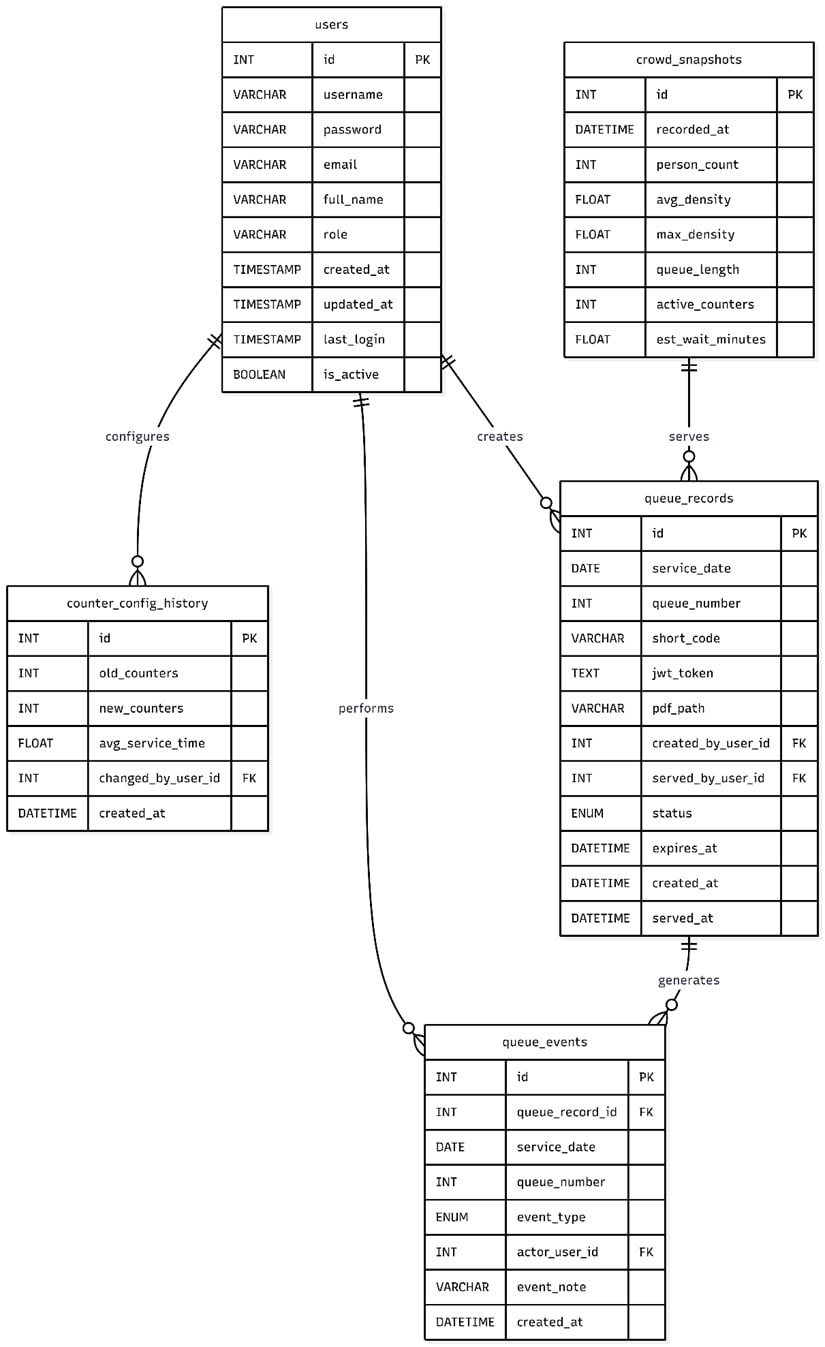
\includegraphics[width=0.85\textwidth, height=0.65\textheight, keepaspectratio]{image/latest ERD.jpg}
    \caption{Entity Relationship Diagram}
    \label{fig:entity relationship diagram}
\end{figure}

\indent\textbf{Data Flow Diagram Level 0}. The data flow diagram illustrates how information flows between the external entities Computer Vision, Students, Thermal Printer, and Administrative Staff and the central Intelligent Queue Management System. It presents the major inputs and outputs exchanged within the intelligent queue management system.

\begin{figure}[H]
    \centering
    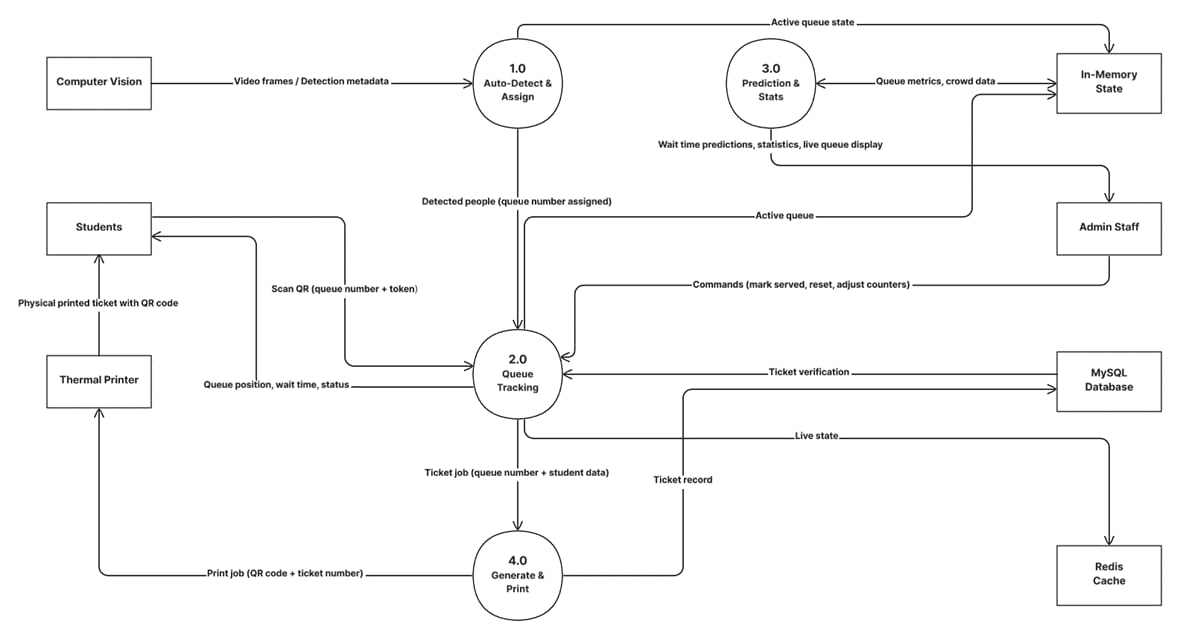
\includegraphics[width=0.85\textwidth, height=0.65\textheight, keepaspectratio]{image/Latest DFD 0.jpg}
    \caption{Data Flow Diagram 0}
    \label{fig:data flow diagram 0}
\end{figure}

The diagram shows the interaction between the four external entities and the IQMS for real-time queue monitoring and wait-time transparency. Computer Vision sends detection payload (tracked people, positions, crowd metrics) to the system. Students interact with the system by scanning QR tickets and requesting queue status information. The Thermal Printer receives print jobs to output physical tickets with QR codes. Administrative Staff sends commands (mark served, reset queue, adjust counters) and receives analytics reports and queue metrics.

\indent\textbf{Data Flow Diagram Level 1}. The Level 1 Data Flow Diagram expands Process 2.0 (Queue Tracking \& Management) into six sub-processes, illustrating how data flows between external entities and the internal processes and data stores of the intelligent queue management system.

\begin{figure}[H]
    \centering
    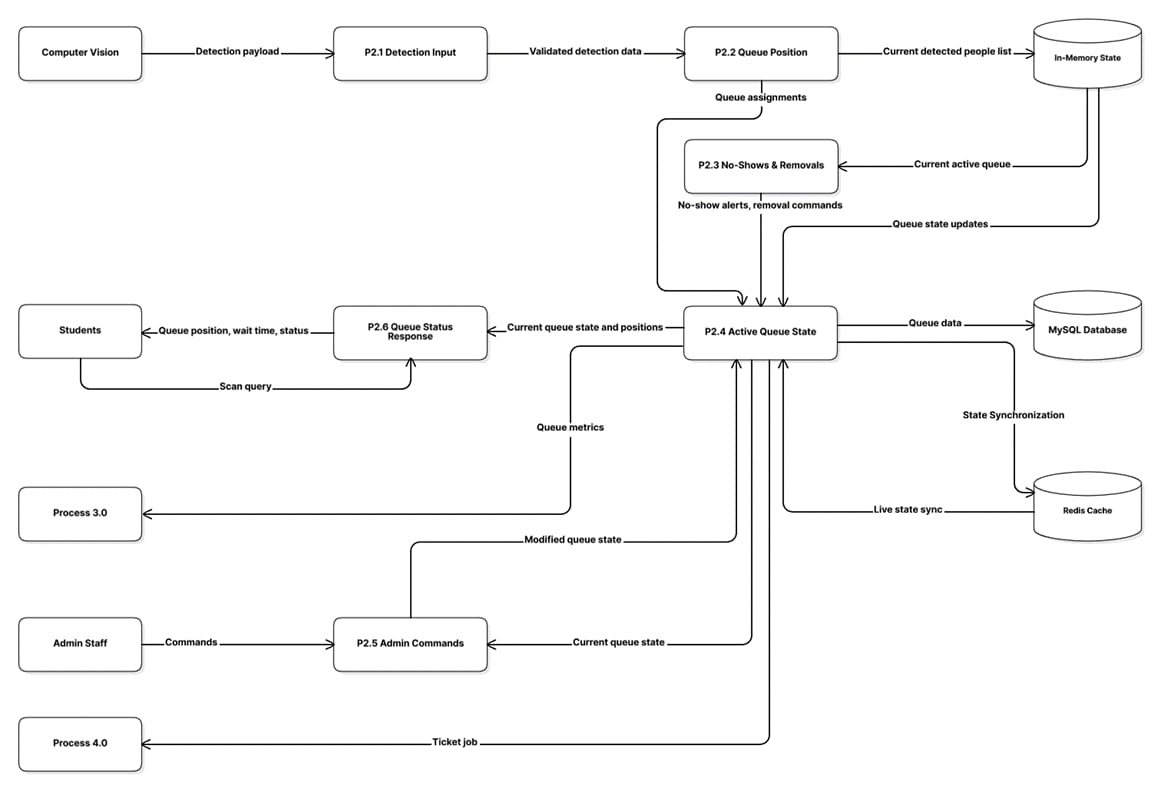
\includegraphics[width=0.85\textwidth, height=0.65\textheight, keepaspectratio]{image/Latest DFD 1.jpg}
    \caption{Data Flow Diagram 1}
    \label{fig:data flow diagram 1}
\end{figure}

\noindent\textbf{P2.1 (Receive Detection Input)} receives video frames and detection metadata from Computer Vision and validates the incoming detection payload.

\noindent\textbf{P2.2 (Assign/Update Queue Position)} takes validated detection data and assigns queue numbers to newly detected students while updating positions for existing students in the queue.

\noindent\textbf{P2.3 (Detect No-Shows \& Removals)} monitors the active queue state and compares it with current detections to identify students who have left the queue or exceeded no-show timeouts, generating removal commands.

\noindent\textbf{P2.4 (Maintain Active Queue State)} serves as the central hub, receiving queue assignments, no-show alerts, and admin commands, then updating and maintaining the live queue state in memory and data stores.

\noindent\textbf{P2.5 (Process Admin Commands)} receives commands from Administrative Staff and processes queue modifications such as marking customers as served or resetting the queue, then communicates changes back to P2.4.

\noindent\textbf{P2.6 (Provide Queue Status Response)} receives queue status queries from Students and returns their current position, estimated wait time, and status.

\noindent The system interacts with three data stores: \textbf{In-Memory State} (stores active queue and snapshots), \textbf{MySQL Database} (stores ticket records and queue history), and \textbf{Redis Cache} (stores live state for cloud deployments and multi-instance synchronization).

\indent\textbf{Architecture Diagram}. The system follows a five-tier architecture designed for integrated visual processing and queue management. The Computer Vision Layer utilizes a Camera and YOLOv8-based detector to extract metadata, which is transmitted via POST requests to a FastAPI-driven Business Logic Layer. Within the backend, a Queue Service and Ticket Printer manage the sequential logic, interfacing directly with a Persistence Layer comprising MySQL, Redis, and In-Memory states to ensure data durability and live synchronization. Automated physical output is handled by a Thermal Printer in the Output Layer to generate QR-coded tickets. User and administrative interactions are facilitated in the Client Layer, where a Flutter application provides real-time status updates and an Admin Web Dashboard offers analytics and manual command overrides.

\begin{figure}[H]
    \centering
    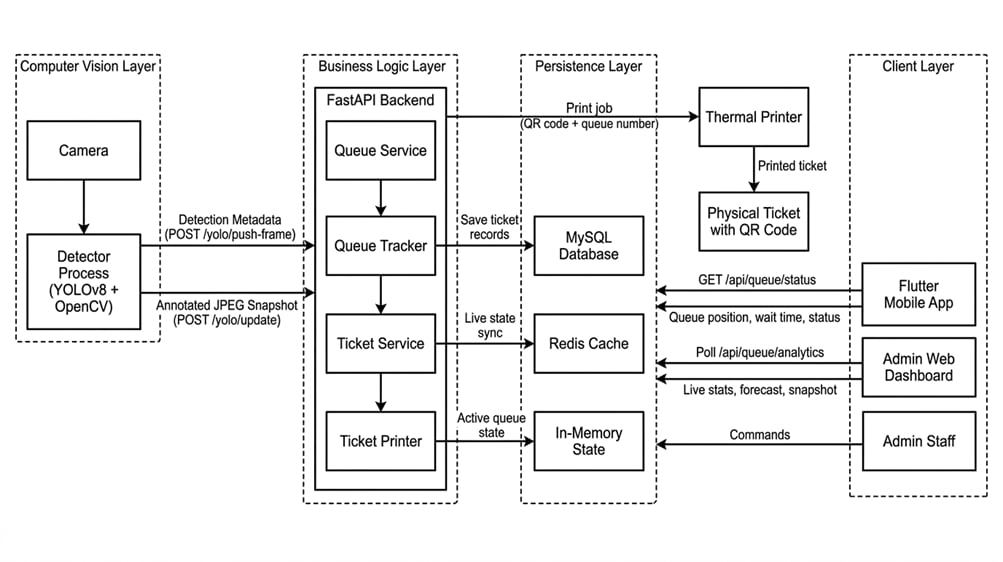
\includegraphics[width=0.85\textwidth, height=0.65\textheight, keepaspectratio]{image/Archi Diagram.jpg}
    \caption{Architecture Diagram}
    \label{fig:architecture diagram}
\end{figure}

\section{Software Development Process}

\noindent This study follows the \textbf{Systems Development Life Cycle (SDLC)} using
the \textbf{Waterfall Model} as the guiding framework for the development of
the Intelligent Queue Management System for Wait Time Transparency. The
Waterfall Model was selected because it provides a clear, structured, and
sequential approach to system development, making it appropriate for an
academic capstone project with defined objectives, a fixed scope, and a
specific institutional setting. Each phase of the SDLC is completed before
the next one begins, ensuring that the system is thoroughly planned, designed,
and evaluated before deployment. This approach also aligns with the
research's overall Design Science orientation, which emphasizes the
systematic construction and evaluation of a working system artifact.
 
The development process follows five sequential phases.
 
\indent\textbf{Requirements Analysis.}In this phase, the researchers identify and document the informational and
operational requirements of the proposed system. Data gathered through
surveys, semi-structured interviews, and direct observation of existing
queueing workflows in the Enrollment and Cashiering offices serve as the
primary basis for defining system requirements. Both functional requirements
--- such as real-time queue tracking, estimated wait-time display, digital
ticket issuance, and administrative notifications --- and non-functional
requirements --- such as system usability, accessibility, reliability, and
data privacy compliance --- are established. Workflow diagrams and process
models are prepared to document the current state of queue operations and
identify areas where the information system can improve transparency and
service efficiency.
 
\indent\textbf{System Design.}Based on the requirements gathered, the researchers produce the system's
design artifacts, including the Entity Relationship Diagram (ERD), Data Flow
Diagrams (DFD Levels 0 and 1), and the overall system architecture. The
design establishes how data will be captured, stored, processed, and
presented across the system's components, covering queue registration,
real-time monitoring, wait-time estimation, notification delivery, and
administrative dashboard reporting. User interface designs for the student
kiosk, mobile application, and administrative web dashboard are developed in
accordance with UI/UX principles for public information displays to ensure
clarity, accessibility, and ease of use for all intended users.
 
\indent\textbf{System Development.}The system is developed based on the approved design specifications. Development
activities include the implementation of the queue management module, the
digital ticketing and QR scanning subsystem, the real-time monitoring and
notification components, the wait-time estimation feature, and the
administrative analytics dashboard. Each subsystem is built in accordance
with the design artifacts produced in the previous phase, and the researchers
coordinate with the institution's IT department to ensure compatibility with
existing infrastructure and institutional workflows.
 
\indent\textbf{Testing and Evaluation.}After development, the system undergoes a series of tests to verify that it
meets the documented functional and non-functional requirements. Testing
covers individual system features, the interaction between system components,
and overall system performance under realistic usage conditions. Feedback
from students, administrative staff, and IT personnel is gathered through
structured evaluation forms to assess usability, functionality, and user
satisfaction. Identified issues are documented and resolved before the system
proceeds to deployment.
 
\indent\textbf{Deployment.}The tested and refined system is deployed at the Enrollment and Cashiering
offices of Naga College Foundation, Inc. for one academic semester during
the 2025--2026 academic year. During this phase, the system is monitored
for operational stability, data accuracy, and user adoption. Performance is
tracked against key indicators, including reductions in average waiting time,
improvements in service throughput, and levels of user satisfaction,
providing the empirical data required for final evaluation and reporting.

\section{Validation and Testing Methods}

\indent\textbf To ensure that the Intelligent Queue Management System meets its intended
informational, functional, and usability requirements, the study employs a
structured validation and testing strategy. Testing is conducted after the
development phase and formally concludes with a user-centered evaluation
involving students, administrative staff, and IT personnel of the institution.
 
\indent\textbf{Functional Testing.}Functional testing is carried out to verify that each system feature performs
in accordance with the documented requirements. Test cases are designed to
confirm that core functions --- including queue registration, digital ticket
generation and QR scanning, real-time queue status display, wait-time
information, automated notifications, and administrative dashboard reporting
--- produce correct and expected outputs under normal operating conditions.
Functional testing also covers scenarios such as simultaneous user
registrations, empty queue states, and manual administrative overrides,
ensuring that the system handles these situations without error or data
inconsistency.
 
\indent\textbf{Integration Testing.} Integration testing examines the correct interaction and data exchange between
the system's interconnected components. Key scenarios evaluated include the
flow of queue data from the monitoring interface to the database and display
screens, the accuracy of wait-time information presented to users, the
end-to-end process from ticket issuance to service completion, and the
consistency of queue records across the kiosk, mobile application, and
administrative dashboard. This level of testing ensures that the system
functions as a unified information system and that no data loss, duplication,
or inconsistency occurs across its integrated modules.
 
\indent\textbf{Performance Testing.}Performance testing assesses the system's responsiveness and stability under
realistic institutional usage conditions, particularly during high-demand
service periods such as enrollment and cashiering deadlines. Scenarios
simulate concurrent user interactions to evaluate system response times for
queue status queries, the timeliness of notification delivery, and the
accuracy and consistency of real-time dashboard updates under load. Results
are compared against acceptable performance benchmarks defined by
institutional service requirements, and identified issues are addressed prior
to full deployment.
 
\indent\textbf{User Acceptance Testing (UAT).}User Acceptance Testing is conducted during the pilot deployment phase to
evaluate whether the system meets the practical expectations and informational
needs of its intended users. Participants --- including students as primary
end users, administrative staff from the Enrollment and Cashiering offices,
and IT personnel responsible for system maintenance --- interact with the
system under supervised conditions and provide structured feedback through
post-evaluation forms aligned with the study's five-point Likert-scale survey
instrument. Qualitative insights are gathered through follow-up interviews to
capture usability concerns, workflow alignment issues, and improvement
suggestions not reflected in quantitative scores. The findings from UAT
directly inform the final refinements to the system before full
semester-wide deployment, ensuring that the delivered information system
effectively addresses institutional needs and enhances the overall queue
management experience.

\clearpage

%-----------------------------
% Chapter 3
%-----------------------------
\chapter{Results and Discussions}

\section{Results}

\subsection{Problem 1}

\subsection{Problem 2}

\subsection{Problem 3}

\section{Design and System Plans}

\section{Summary of Findings}

\section{Conclusions}

\section{Recommendations}

%-----------------------------
% References
%-----------------------------

\clearpage

\printbibliography

\clearpage

\chapter*{Curriculum Vitae}

\chapter*{Appendices}

\end{document}
